\subsection{Muon System}

The forward muon arm has been described in ~\cite{Aamodt:2008zz} . It consists of a
composite absorber ($\sim 10\ \lambda_{int}$), made with layers of
both high- and low-Z materials starting 90 cm from the mean
interaction point, a large dipole magnet with a 3 Tm integrated field
placed outside the L3 barrel magnet, and ten planes of very thin, high
granularity, cathode pad tracking stations. A second muon filter
($\sim 7\ \lambda_{int}$ of iron) at the end of the spectrometer and
four planes of Resistive Plate Chambers are used for muon
identification. The spectrometer is shielded by a dense conical
absorber tube, of about 60 cm outer diameter, which protects the
chambers from secondary particles created in the beam pipe.

The increase of luminosity of the LHC after LS2 requires an upgrade of
the front-end and read-out electronics on both muon
tracking and muon identifier subsystems.


\subsubsection{Muon Tracking}

The Muon Tracking Chambers (MCH)~\cite{Aamodt:2008zz} was operated
during LHC run~1 and run~2. It is based on 156 multi-wire proportional
chambers with cathode pad readout, the so called Cathode Pad Chambers with more than
one million electronic channels. 
The system consists of 5 tracking stations, each of which is composed of 2
chambers. Because of the different sizes of the stations, (ranging from few square metres for station 1 to more than 30 m$^{2}$  for station 5) two different designs were adopted. The first two stations are based on a quadrant structure ~\cite{Peyre}, with the readout
  electronics distributed on their surface (see Figure ~\ref{quad+slat} (Left) ). Four independent quadrants constitute one chamber. For the larger stations (3 to 5), a slat architecture ~\cite{Cicalo} was chosen (see Fig. ~\ref{quad+slat} (Right)). The maximum
  size of a slat is 40 $\times$ 240 cm$^{2}$ and the electronics are mounted on the top and bottom part of
  each slat. Slats are mounted on a support to constitute one
  half-chamber. One half-chamber consists of 9 slats for station 3,
  and 13 slats for stations 4 and 5. The tracking system
  covers a total area of about 100 m$^{2}$. 

\begin{figure}[h]
  \centering
  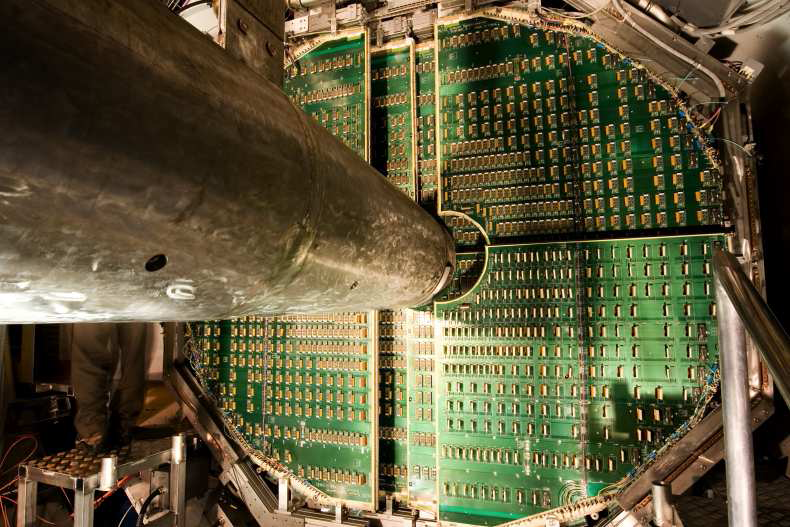
\includegraphics[width=.45\textwidth]{mch/quadrant.png}
  \hspace{0.05\textwidth}
  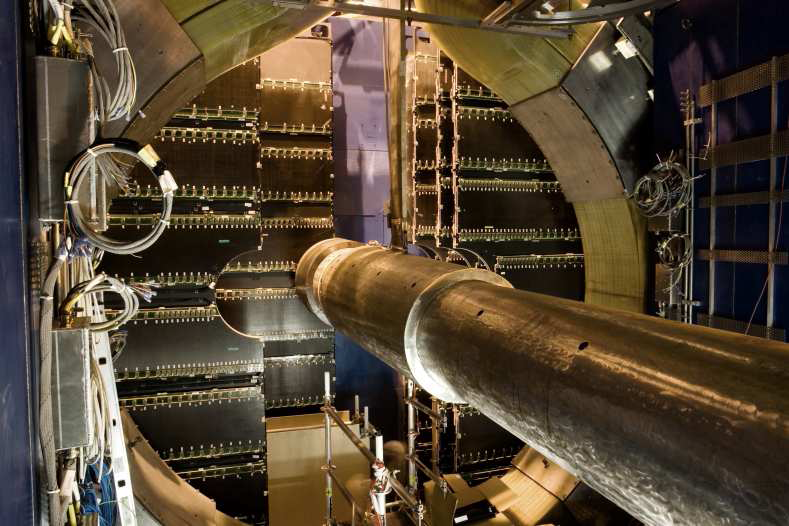
\includegraphics[width=.45\textwidth]{mch/slat.png}
   \caption[Tracking system layout]{Left: Layout of station 2 of the tracking system; the readout electronics is distributed on the surface of a quadrant. Right: Layout of stations 4 and 5 of the tracking system; the readout electronics are mounted along the top and bottom edge of the slats.}
  \label{quad+slat}
\end{figure}

Due to the increase of luminosity of the LHC after LS2, the front-end
and the readout electronics have been upgraded, keeping the detectors
unchanged.

The electronics can run either in trigger or in our default dead time free continuous
mode. The data flow readout scheme is shown in
Fig.~\ref{readoutscheme}. The Front-end Cards (FEC) send continuously words through an electrical link at 80 Mbit/s to the SOLAR
read-out board which connects to the Concentrator Readout Unit (CRU)
through GBT optical link at 3.2 Gbits/s.

\begin{figure}[h]
  \centering
  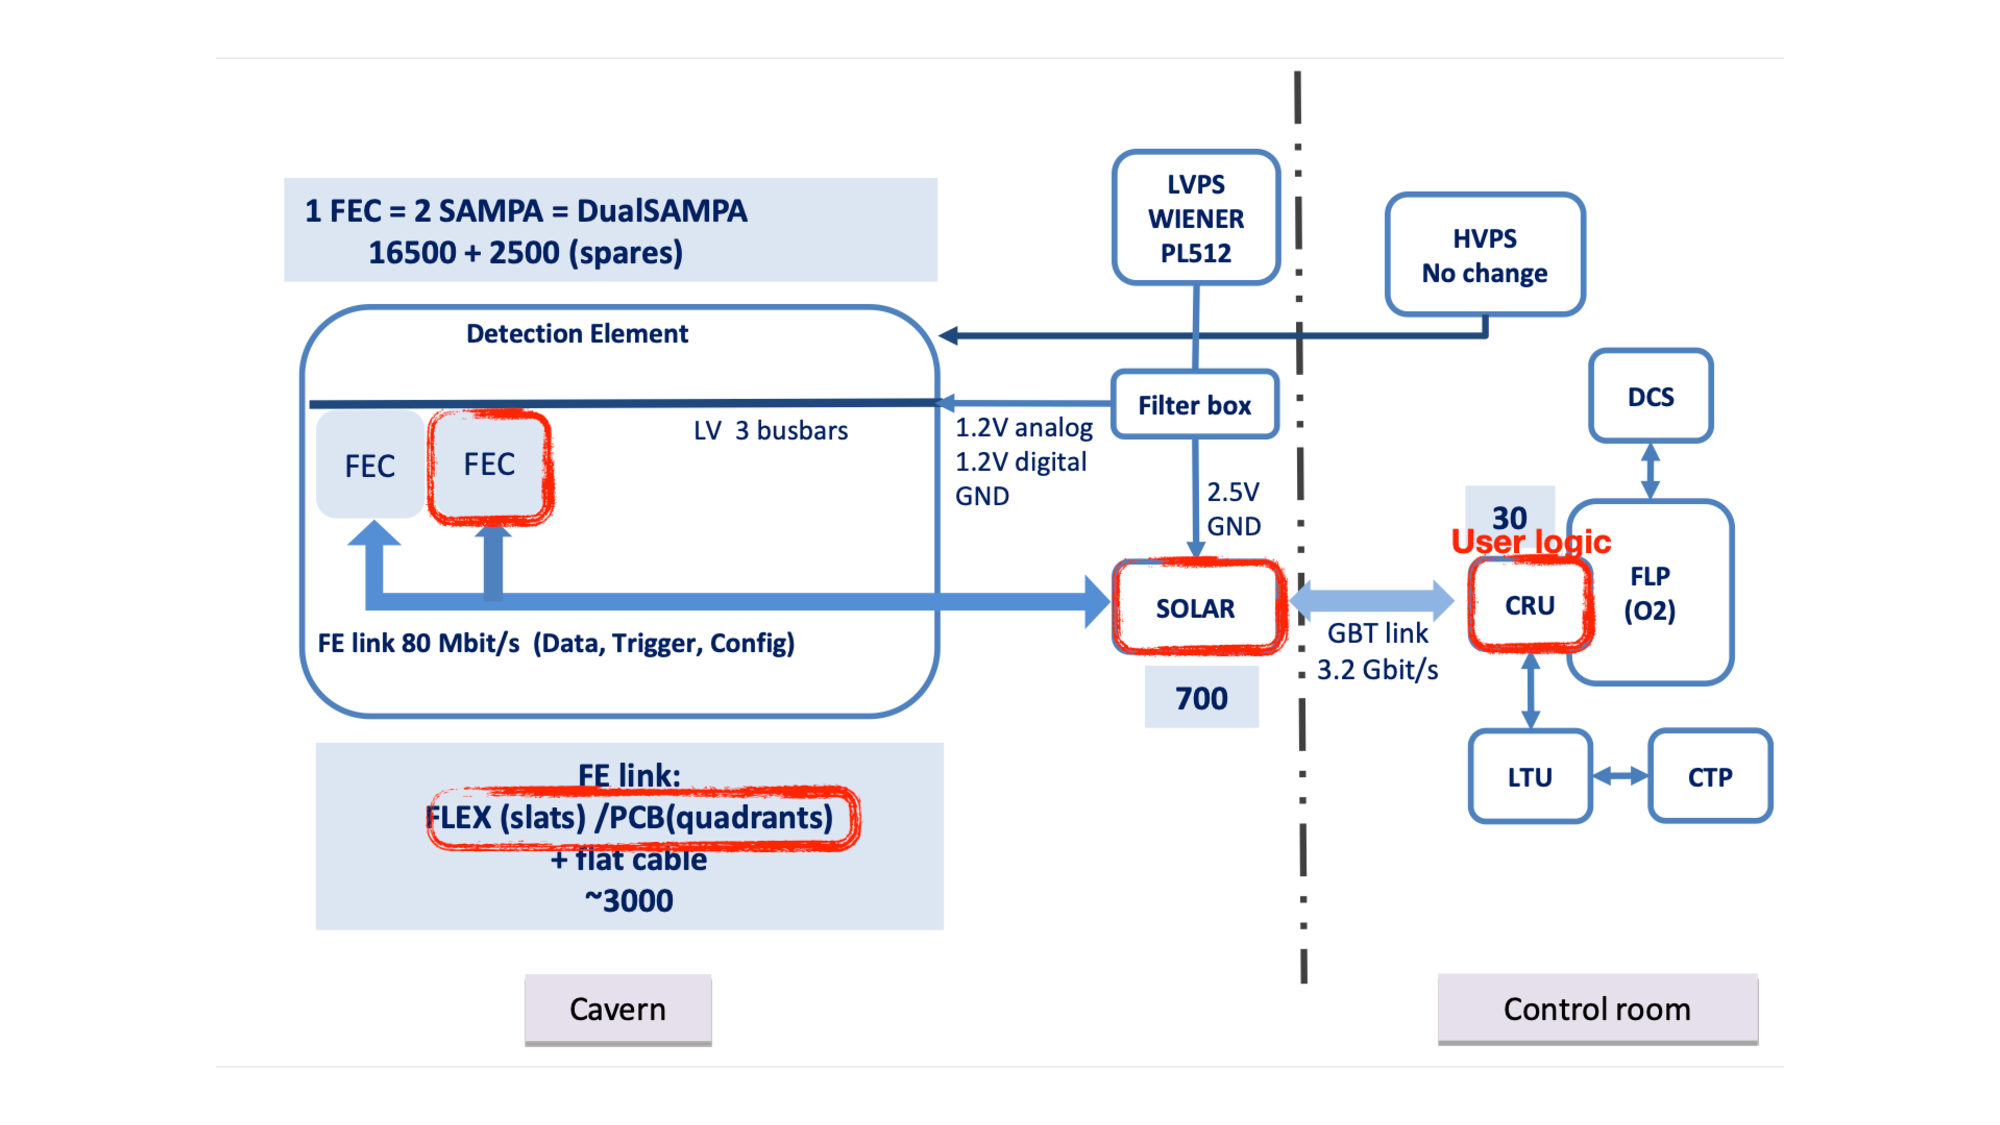
\includegraphics[width=1\textwidth]{mch/readoutscheme.pdf}
     \caption[Tracking readout scheme]{ The Muon Tracking readout scheme}
  \label{readoutscheme}
\end{figure}

\paragraph{The DualSAMPA front-end electronic cards\\}

The front-end electronic cards, called DualSAMPA, host 2 chained SAMPA chips (
see chapter 3.2) of 32
channels each and 3 low voltage regulators. Since the detectors are not
changed, the dimensions and the layout of the connectors for the DualSAMPA cards on the
electronic PCBs remain the same as for the previous FEC. Moreover, two
types of cards were produced, each with the same functionalities but with
different dimensions to cope with the two detector types, quadrant and
slat (see Fig.~\ref{dualsampa}).

\begin{figure}[h]
  \centering
  \includegraphics[width=1\textwidth,height=8cm]{mch/dualsampa.pdf}
     \caption[DualSAMPA]{ The two geometries of the DualSAMPA boards,
       with the white connector plug socket on PCB and on the
       other side the black connector connecting to the electrical link. }
  \label{dualsampa}
\end{figure}


Out of the 19300 DualSAMPA produced (11000 DS345 for slats of stations 3,4 and
5 and 8300 DS12 for quadrants of stations 1 and 2), 16900 are
installed in the cavern (9700 DS345, 7200 DS12).

\paragraph{The readout electronic FLEX links and large electronic PCBs\\}

The link between the DualSAMPA and the readout cards consists of a
flexible circuit (FLEX) and a flat ribbon cable for the slats while a
large electronic PCB and a flat ribbon cable is used for the quadrants (see
Figs.~\ref{flex+pcb}(Left) and ~\ref{flex+pcb} (Right)).

\begin{figure}[h]
  \centering
  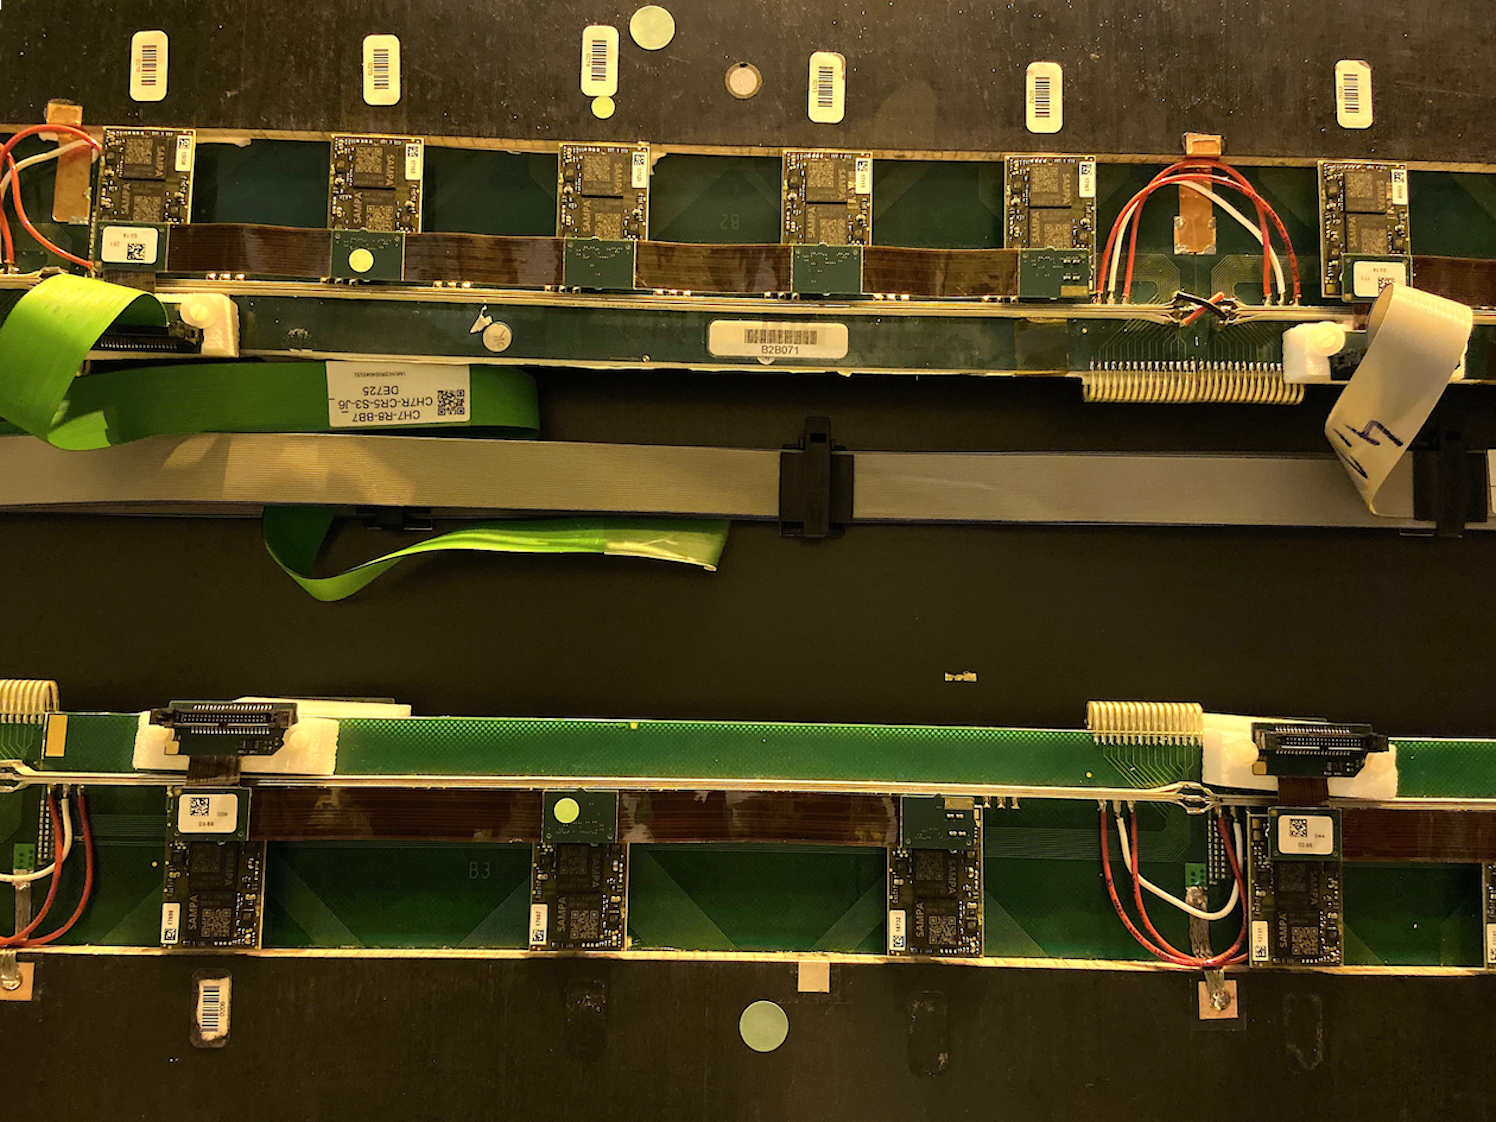
\includegraphics[width=.45\textwidth,height=5cm]{mch/flex.png}
  \hspace{0.05\textwidth}
  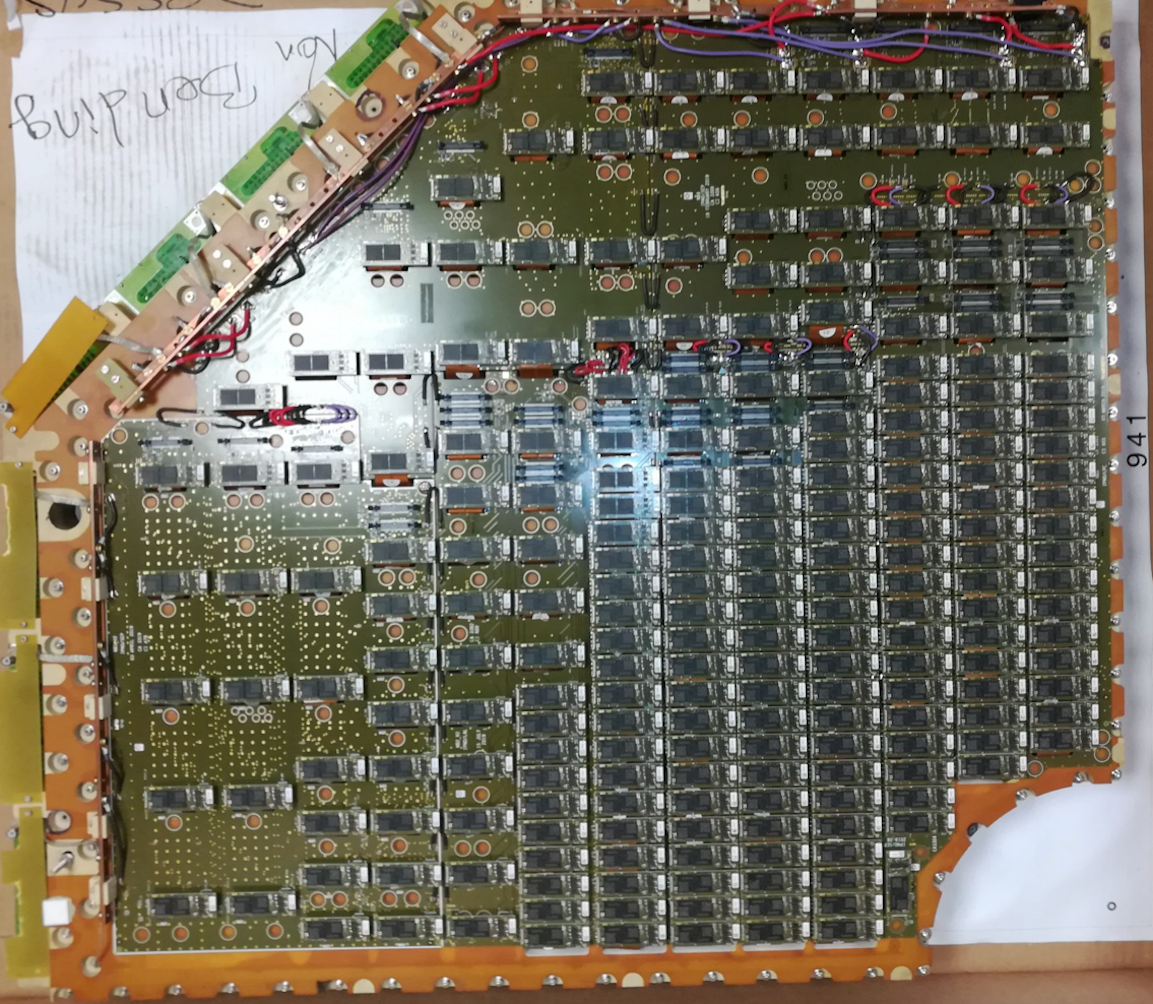
\includegraphics[width=.45\textwidth,height=5cm]{mch/largepcb.png}
   \caption[Electronic links]{Left:Flex mounted on a slat connecting 5
     DualSAMPA cards linking through a green flat ribbon cable with the readout
     board. Right:Large electronic PCBs covering the surface of a quadrant.}
  \label{flex+pcb}
\end{figure}

Each DualSAMPA has dedicated data and clock lines while the
trigger lines are daisy chained to feed up to 5 DualSAMPA (see
Fig.~\ref{flexscheme}). A I2C line allows to address up to 5
DualSAMPA. An active buffer was added to the I2C line to insure a
good signal integrity.

More than 3000 FLEX were produced, of 24 different types depending on the number of DualSAMPA
to address, the geometry and pad density; among them 2760 were
installed.
 
\begin{figure}[h]
  \centering
  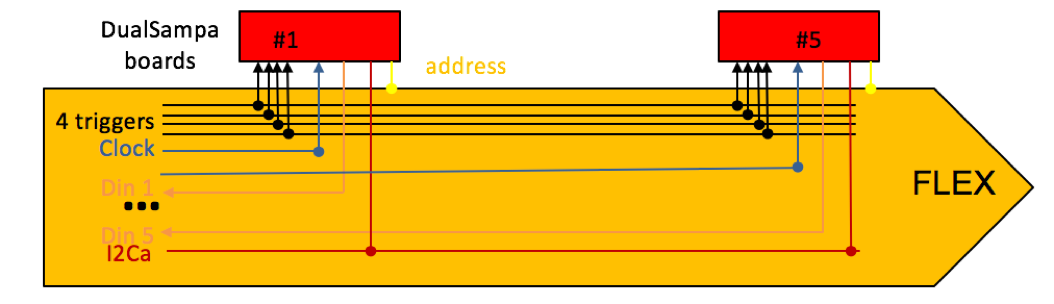
\includegraphics[width=0.8\textwidth, height= 4cm]{mch/flexscheme.png}
     \caption[FLEX scheme]{ The FLEX scheme}
  \label{flexscheme}
\end{figure}



\paragraph{The SOLAR readout cards\\}
Each FLEX/ribbon cable is plugged into one of the 8 ports of the SOLAR readout
board, allowing this latter to read out up to 40 DualSAMPA boards (see
Fig.~\ref{solarscheme}). The GBTx chip of the SOLAR
board acts as a deserializer of the  signal coming from the DualSAMPA
and a serializer to send the signals from the different FEC to the CRU through GBT optical
links. The SOLAR board hosts also a GBT-SCA chip handling the 8 I2C
command/control lines, one optical transmitter/receiver VTRx and 2
DC/DC FEAST converters. 
 
\begin{figure}[h]
  \centering
  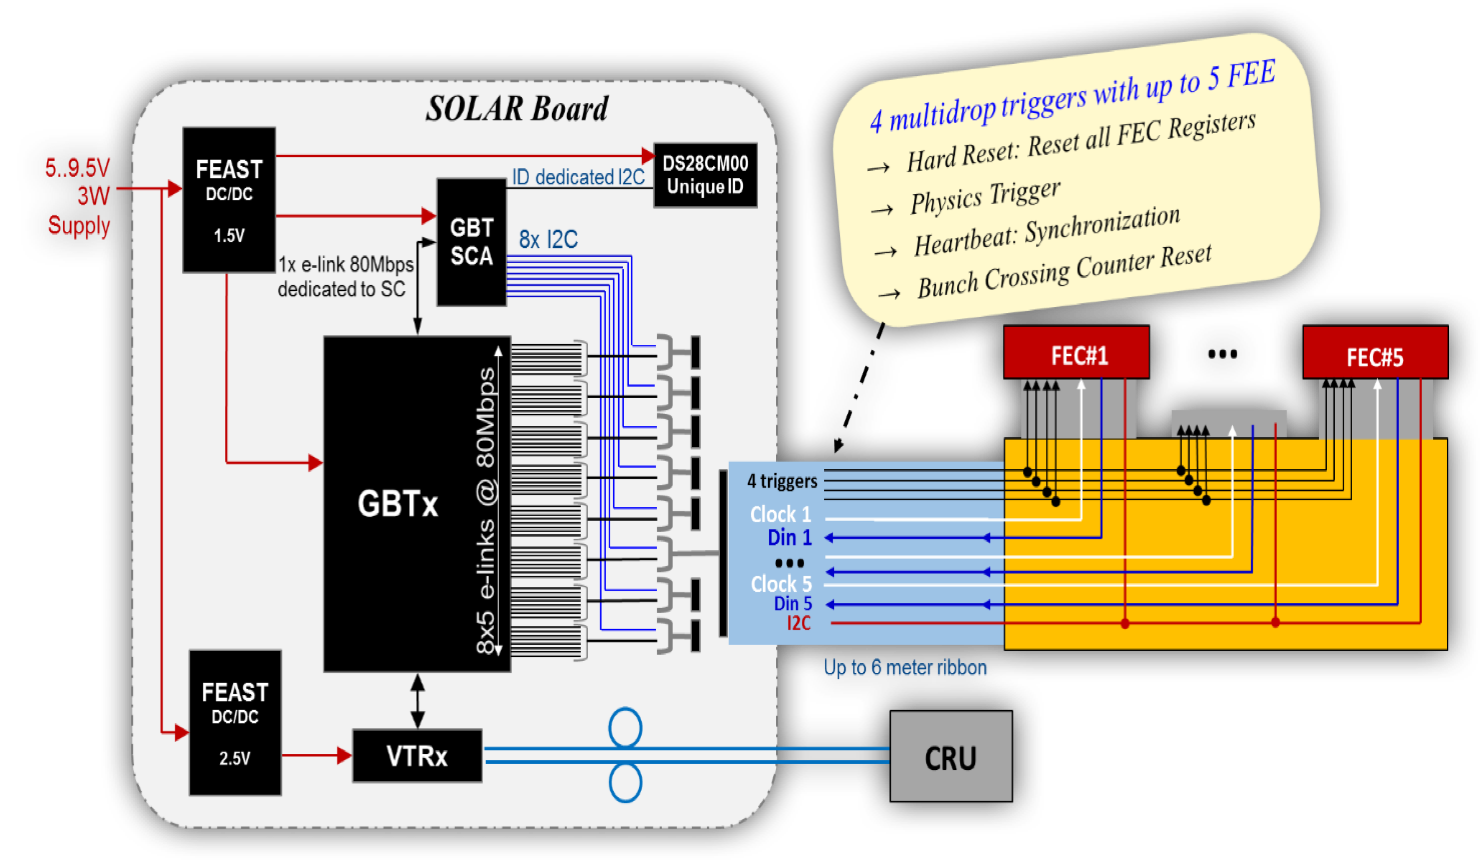
\includegraphics[width=1\textwidth]{mch/solarscheme.png}
     \caption[SOLAR scheme]{ The SOLAR scheme}
  \label{solarscheme}
\end{figure}

The 624 boards produced are placed in 112 custom SOLAR crates, each
one hosting up to 6 boards.


\paragraph{The data flow from SAMPA to the CRU User Logic\\}
In the SAMPA chip, the signal of each electronic channel is amplified with a ~4mV/fC gain,
waveformed with a shaping time of 300 ns, then sampled and digitized at 10 MHz in
a 10-bits ADC and is finally digitally processed with a baseline
correction and a zero-suppression before being formatted. The SAMPA format
consists of data samples from a signal waveform with its time stamp and
size together with a header containing mainly the bunch crossing number, the SAMPA
address and the channel address of the SAMPA chip.

 The signals of the 64 channels of
the two-chained SAMPA chips of a FEC are serialized at 80
Mbits/s (2bits at 40 MHz). The first port of the SOLAR board handles
the first 2 bits of the first DualSAMPA while the second port takes care of the 2 bits of
the second DualSAMPA and so on up linking all 40 ports whihc results in a 4.2
Gbits/s data optical transmission to one input of a CRU. The
electrical and optical links are always sending words, whatever the
type of information (physics data, synchronisation (SYNCH), ...). 

The MCH CRU User Logic (UL) receives data from the 24 GBT links (see description of the CRU in
chapter 6.3), each one handling 40 DualSAMPA channels. For each GBT
link, the UL deserializes the 80 bits, forms the SAMPA
words, remove the SYNCH words and inserts error checks and
condition. The 64 bits SAMPA words contain the payload, the GBT
link identifier, the DualSAMPA channel identifier, and error bits. The
UL then embeds the TTC signals into the stream, constructs
the RDH (Redaout Data Header) and transmits words of 256 bits to the FLP (Front Level
Processor) (see Fig. ~\ref{dataflow} and~\ref{cru-ul}).

\begin{figure}[h]
  \centering
  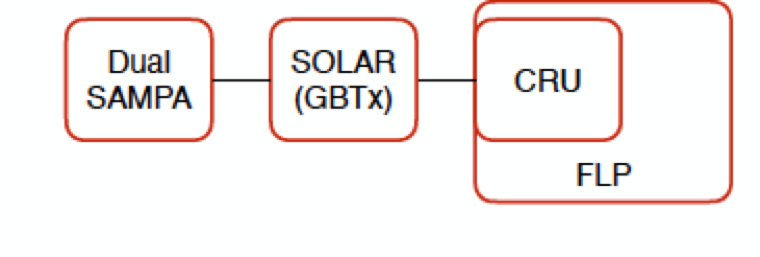
\includegraphics[width=0.7\textwidth,height=3cm]{mch/dataflow.png}
     \caption[Data flow]{Data flow scheme}
  \label{dataflow}
\end{figure}

\begin{figure}[h]
  \centering
  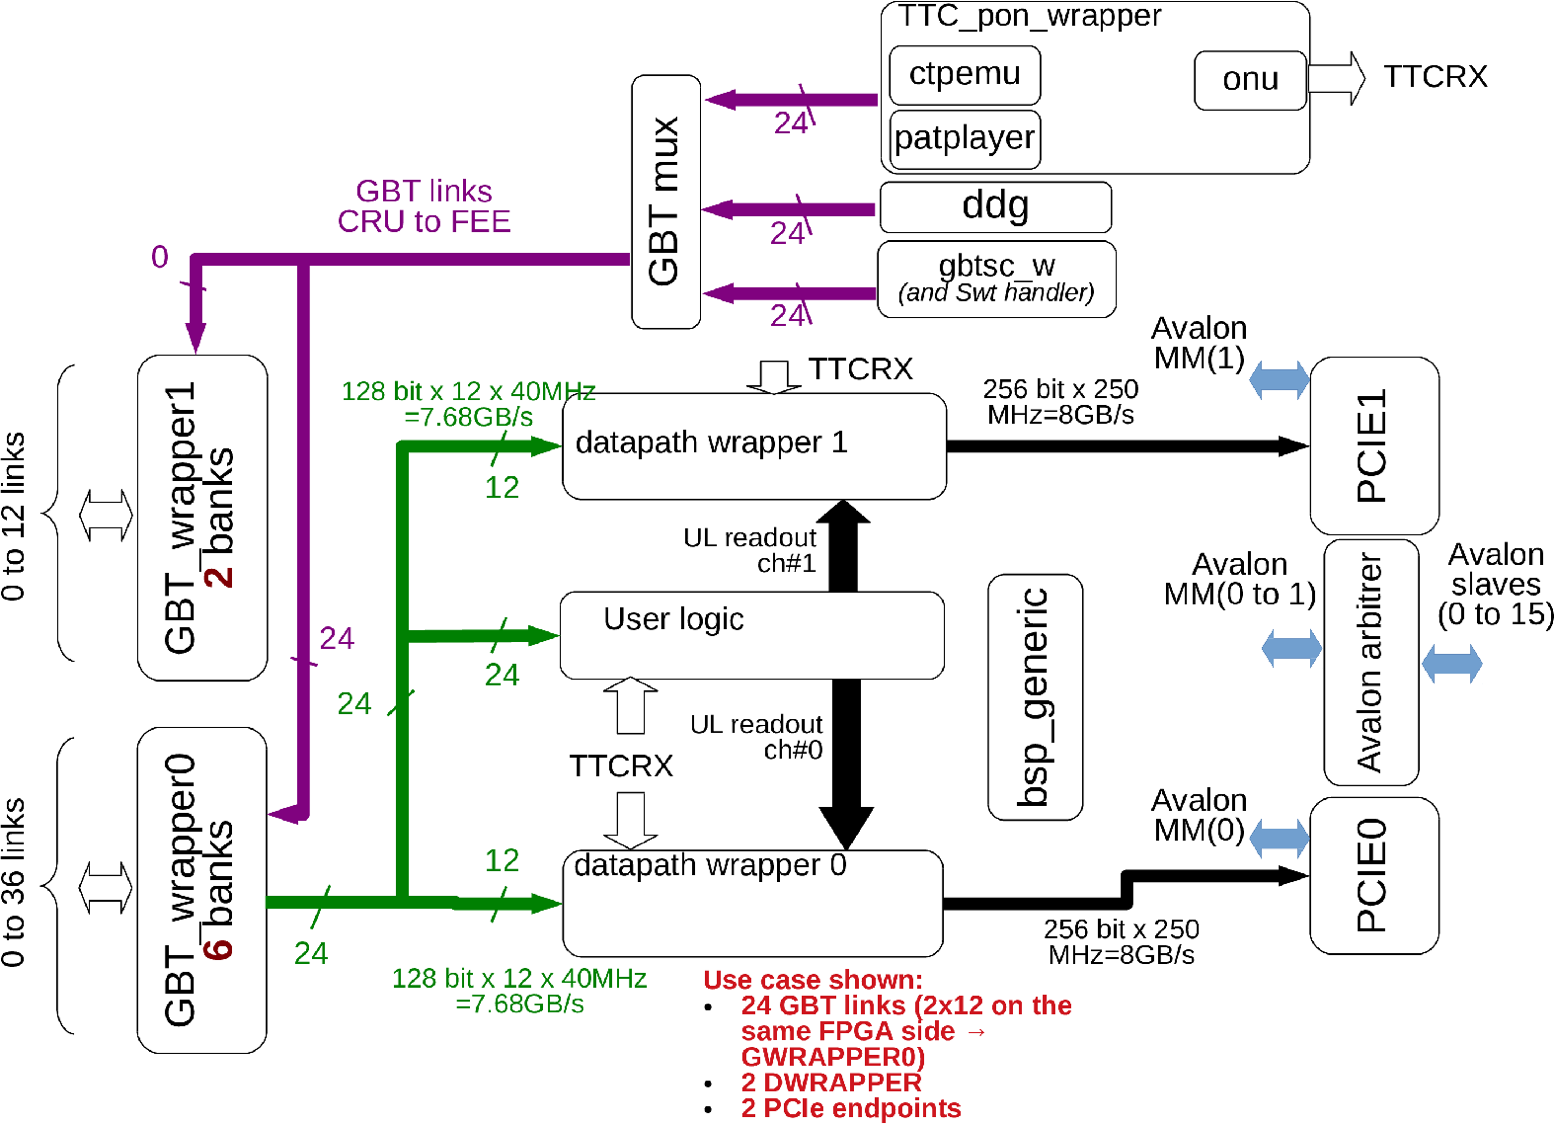
\includegraphics[width=1\textwidth]{mch/cru-ul.png}
     \caption[CRU Scheme]{CRU scheme}
  \label{cru-ul}
\end{figure}

The $O^2$ processes, carried out on FLPs or/and EPN,  will perfom the decoding of the data
format received from the CRU, the pre-clustering, clustering and tracking. These
will also run the simulations.
During data taking the Quality Control (QC) processes data samples for detector performances
monitoring.



\subsubsection{Muon Identifier}

The Muon Identifier (MID) is the present designation of the Muon Trigger system~\cite{Aamodt:2008zz} which was operational in ALICE during LHC run~1 and run~2. 

The detector is composed of 72 single gap Resistive Plate Chamber (RPC) detectors, organized in two stations of two planes each, located at 16~m and 17~m from 
the interaction point. The planes in the same station are 17~cm apart. The total detection area is about 150~m$^{\rm 2}$. An overview picture of one half-plane of the MID, in open position, taken during the FEERIC card 
installation (see next section) in 2019, is shown in Fig.~\ref{midhalfplaneopen}.

The RPC signals are collected by means of a total of 20992 readout strips, each of them equipped with Front-End (FE) electronics. The output signals from the FE electronics, in LVDS electrical standard of 25~ns width, 
are propagated via multi-wire copper cables to the readout electronics (also in charge of the muon trigger decision during run~1 and run~2). 

\begin{figure}
\centering 
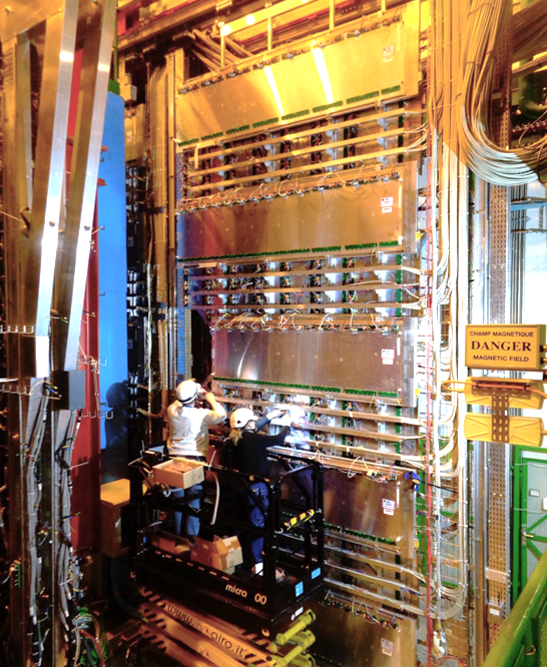
\includegraphics[width=.4\textwidth]{mid/midhalfplaneopen}
\caption{Overview of one MID half-plane in open position}
\label{midhalfplaneopen}
\end{figure}

The FE electronics cards, located on the RPC detectors, have been replaced during the LS2. The main motivation is to reduce the ageing of the RPCs during future data taking periods. 
The FE ASIC of the past FE electronics, called ADULT~\cite{mid:ADULT}, has been upgraded to a new one, called FEERIC~\cite{mid:FEERICref1,mid:FEERICref2}.
Unlike ADULT, FEERIC performs amplification of the RPC analog signals. Thanks to this upgrade, the ALICE RPCs will be operated in avalanche 
mode after the LS2 with a significant reduction of the charge produced in the gas gap as compared to past conditions, hence limiting ageing effects.

The readout electronics (more than 250 complex electronics cards) have been also completely replaced for sustaining the large data flow going with the future high collision rate. 
The new system is designed for continuous readout so there is no more need for hardwired muon trigger signals, the event selection being done at the online processing level. 

All RPC detectors were still operational at the end of run~2. However few of them were drawing a relatively large current after having accumulated up to 20~mC/cm$^{\rm 2}$.
It was therefore decided to replace those RPCs by completely new produced ones. For the longer term, a crucial R\&D on new environment-friendly 
gas mixtures~\cite{mid:RPCgasmix} for RPCs, based on tetrafluoropropene which is characterized by a very low Global Warning Potential (GWP), has been launched.


\paragraph{FEERIC electronics\\}
 
The FEERIC 8-channel ASIC is designed in the AMS 0.35~$\mu{\rm m}$ CMOS technology. It is mostly composed (see Fig.~\ref{midFEERIC}, top scheme) of a transimpedance amplifier, a zero-crossing discriminator and a one-shot 
which prevents retriggering during 100~ns. The operating threshold is typically 70~mV corresponding roughly to 130~pC at readout strip level. Details of the performance of the FEERIC electronics 
is given in~\cite{mid:FEERIC-PRR}. Figure~\ref{midFEERIC}, bottom, shows a picture of a FEERIC card. 2720 cards (spare included) have been produced in the second half of 2017.
The installation of the FEERIC cards on the RPCs in ALICE cavern has been completed in July 2019. 

In parallel, a new wireless threshold distribution for the FEERIC cards has been developed. 
A total of two masters (one per side of the cavern) and 24 nodes close from the RPCs (see Fig.~\ref{midTHRdistri}, picture on the right), installed in ALICE cavern in 2019, allows to remotely control the threshold of each of the 2384 installed 
FEERIC cards. The masters are controlled via ethernet and communicate via the high level ZIGBEE wireless protocol with the nodes which are themselves I2C chained to the FEERIC cards on the RPCs (see Fig.~\ref{midTHRdistri}, 
scheme on the left). Master and node share the same hardware and firmware. Card acts as master or node depending on the configuration stored in EEPROM which also keep memory of the last requested threshold values, restored
at power on.  

During run-2, one of the 72 ALICE RPCs was equipped with FEERIC electronics and the wireless distribution, showing satisfactory performance and stability. The charge released in the gas (25-30~pC per hit) is four times less 
than the one of RPCs with ADULT.

\begin{figure}
\centering 
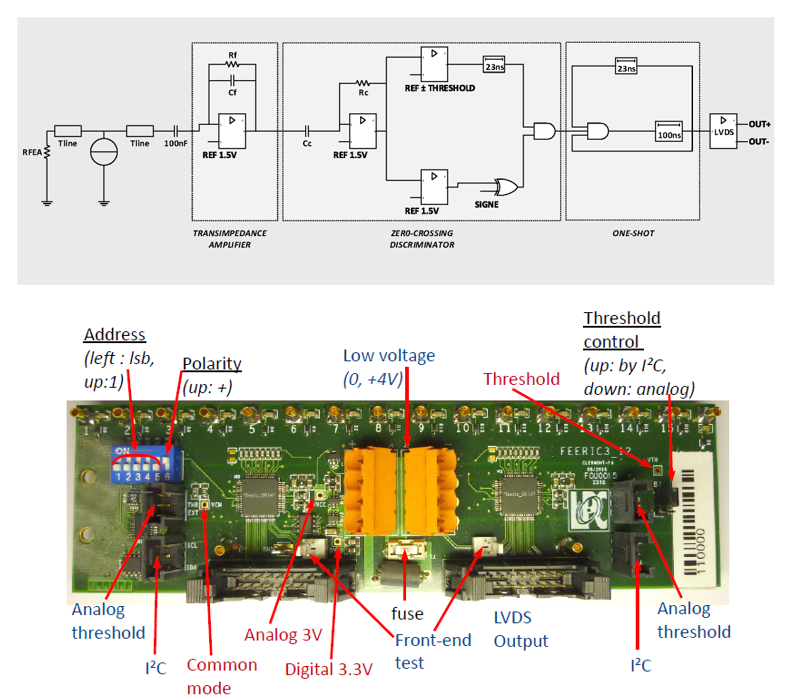
\includegraphics[width=.5\textwidth]{mid/midFEERIC}
\caption{FEERIC ASIC architecture (top) and FEERIC card picture (bottom)}
\label{midFEERIC}
\end{figure}

\begin{figure}
\centering 
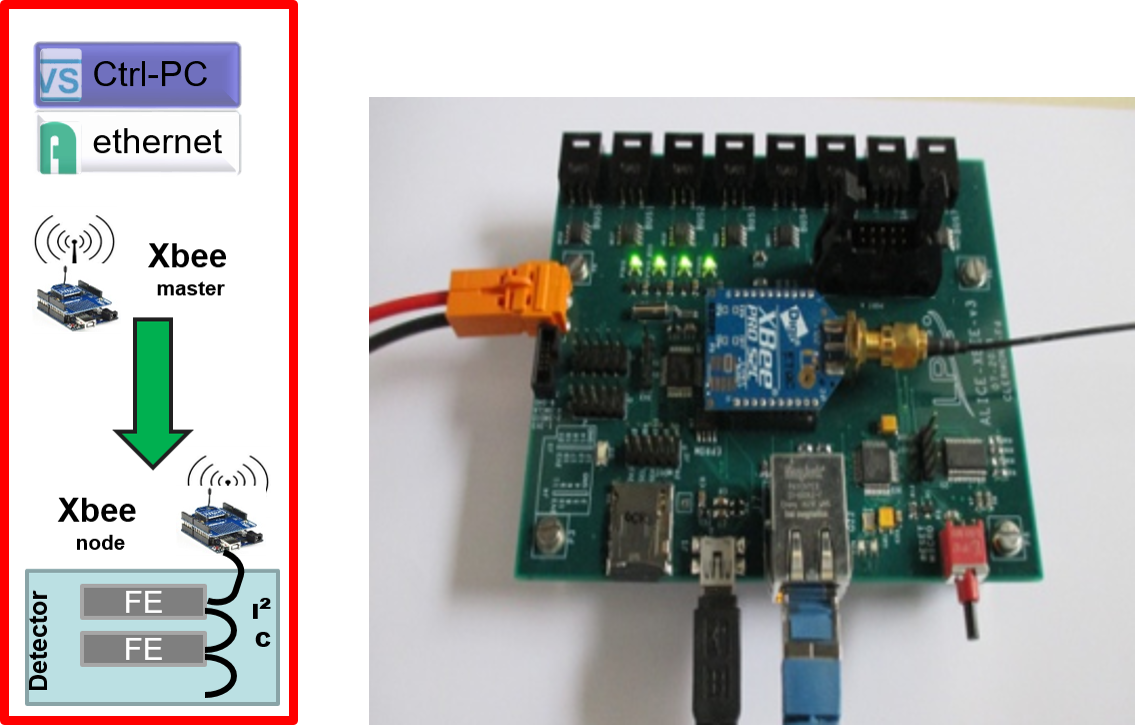
\includegraphics[width=.5\textwidth]{mid/midTHRdistri}
\caption{Wireless threshold distribution scheme (left) and master or node electronics card (right)}
\label{midTHRdistri}
\end{figure}




\paragraph{Readout electronics\\}

The LVDS (binary) signals from the FE electronics, so called strip-patterns of length 16 bits, are received by the Local cards. 
Each Local receives strip-patterns from the four detector planes, each of them from the two orthogonal coordinates (from horizontal and vertical readout strips on both sides 
of the same RPC). The whole project consists in 234 Local cards, housed in 16 VME-9U crates used as mechanical support and for power supply. 
The Regional card in the crate communicates with a maximum of 16 Local cards via the e-links of the J2 bus. Each Regional card is interfaced to a Common Readout Unit (CRU) by means of two GBT links at 3,2~Gbit/s. 

The project has a total of two CRUs only, housed in one single First Level Processor (FLP) tower PC. The MID readout architecture is shown in the left panel of Fig.~\ref{midRO} while a picture of the three types of readout cards 
is shown on the right. Simulations of the expected bandwidth for Pb--Pb collisions at 50~kHz, based on run~2 real data, indicate that 
this design includes a safety factor of more than one order of magnitude. 

Data corresponding to so-called self-triggered physics events~\cite{mid:ROweb,mid:DataNote} are transmitted from the Local and Regional to the CRU. There is potentially a new event stored 
in the Local and Regional FIFOs each 25~ns. Information is stored in these FIFOs only in case of a non-empty event which, in standard configuration,
corresponds to at least two coordinates in the same detector plane with non-zero bit-patterns. 
It is important to note that it takes five clock cycles (at 40~MHz) per self-triggered event for the transfer of the Regional FIFO and 9-21 clock cycles for the transfer of the Local FIFO, depending on the
number of non-empty planes in this last case. As a first consequence, the data from Local and Regional corresponding to the same bunch crossing (BC) arrive asynchronously in the CRU. As a second consequence, the
Local and Regional FIFOs would go to saturation in case of filling at the full clock frequency, corresponding for example to a very high level of noise at the FE level: a busy bit would be set in such case.

The CRU user logic (UL), first stage of data processing in the CRU, is essentially performing zero-suppression and raw data header construction using the central trigger (CTP) orbit information. 
The UL output is transmitted by words of 256 bits to the FLP. At this level, the data coming from the different GBT links are assembled in C++ structures and synchronized to provide the information 
corresponding to a given interaction. The readout electronics always operates in continuous readout mode. However the system can also handle triggered mode, selecting those events in coincidence with a trigger from the CTP, either 
in the CRU or the FLP.

The Local and Regional respond (see~\cite{mid:ROweb}) also to all types of central triggers issued by the CTP and received via the GBT down-link. 




\begin{figure}
\centering 
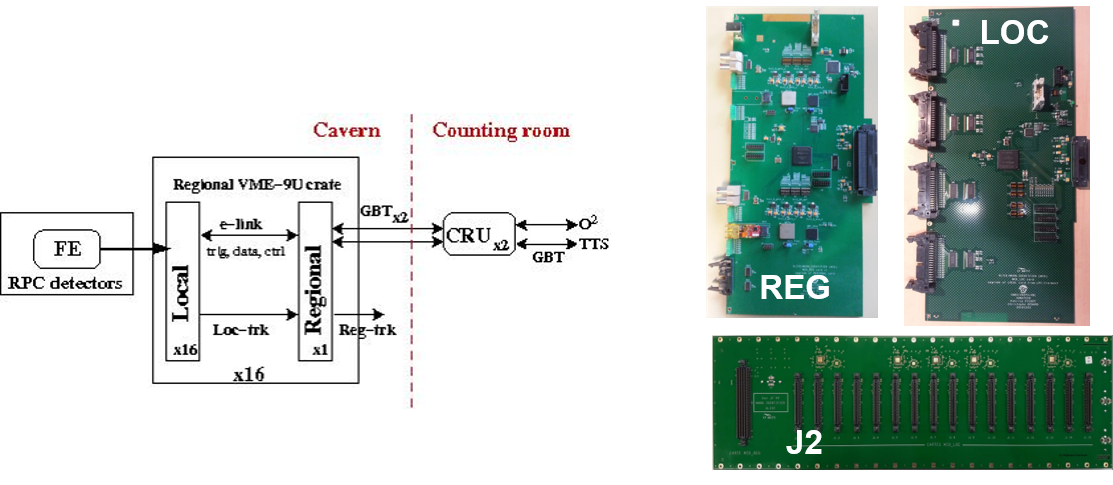
\includegraphics[width=1.\textwidth]{mid/midRO}
\caption{MID readout architecture (left) and readout cards (right picture) with Local (top right), Regional (top left) and J2 bus (bottom ) between Local and Regional}
\label{midRO}
\end{figure}





